\documentclass[../DS03.tex]{subfiles}%
\graphicspath{{./figures/}}%

%\subimport{/home/nora/Documents/Enseignement/Prepa/bpep/exercices/TD/plateforme_mer/}{sujet.tex}

\begin{document}%

\section[52]"P"{Mouvements d'une plateforme
\textit{offshore}\ifcorrige{~\small\textit{(CCP modélisation 2019)}}}
\enonce{%
	On s'intéresse à la résolution d'une équation du mouvement dans une approche
	classique de la mécanique afin d'étudier le mouvement simplifié d'une plateforme
	en mer. Le modèle envisagé est un système à un degré de liberté considéré comme
	un oscillateur harmonique : une masse est reliée à un ressort, avec
	amortissement.
	\bigbreak
	On considère le mouvement d'une plateforme en mer soumise à un courant marin. Sa
	partie supérieure de masse $m = \SI{110}{tonnes}$ est considérée comme rigide et
	le mouvement principal de la plateforme a lieu suivant $x$ (cf figure 1(a)).
	\begin{center}
		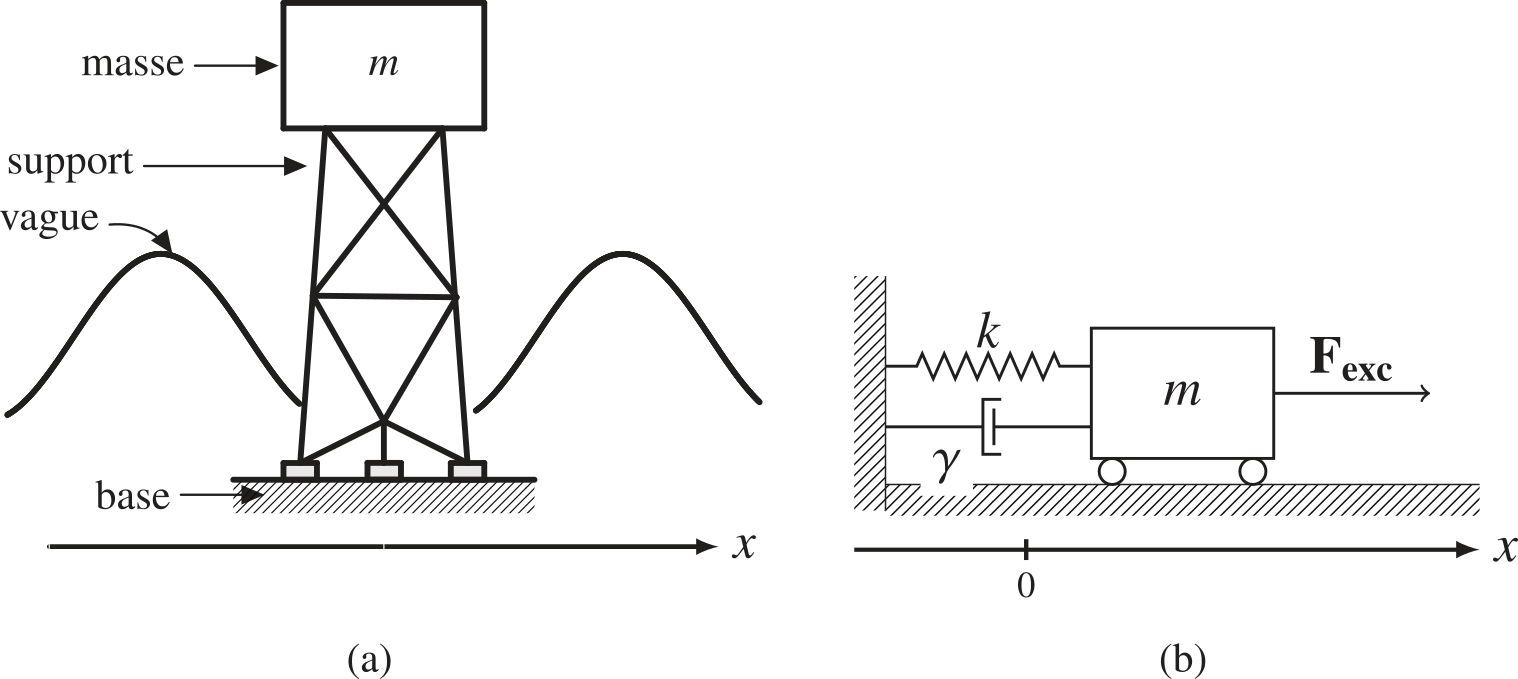
\includegraphics[width=.9\linewidth]{P2_enon}
	\end{center}
	Afin d'étudier le mouvement de cette plateforme, on la représente par une masse
	$m$, liée à un ressort de constante de raideur $k$ et à un amortisseur de
	constante d'amortissement $\gamma$ comme schématisé sur la figure 1(b). La masse
	se déplace selon une seule direction, parallèle à l'axe $Ox$ en fonction du
	temps $t$.
	\bigbreak
	Ainsi, les projections sur l'axe $Ox$ de la position, de la vitesse et de
	l'accélération de la masse en fonction du temps sont notées
	respectivement $x(t)$, $\dot{x}(t)$ et $\ddot{x}(t)$. Le vecteur unitaire de
	l'axe $Ox$ est noté $\ux$.
	\bigbreak
	La masse se déplace sur la base horizontale sans frottements sur le support.
	La position d'équilibre de la masse sera choisie à $x = 0$.
	\bigbreak
	La force totale $\vv{F_{tot}}$ agissant sur la masse correspond à la réaction
	normale à la base horizontale $\vv{R_N}$, à la force de frottement
	$\vv{F_d}= - \gamma \vv{v}$ où $\gamma$ est la constante d'amortissement
	positive, permettant  de prendre en compte l'effet de l'eau environnante, à la
	force de rappel $\vv{F_k}$ du ressort et au poids $\vv{P}$ de la masse $m$.
	\begin{tcn}(tool)<lftt>{Outils mathématiques}
		\[
			\cos(a+b)=\cos(a)\cos(b)-\sin(a)\sin(b)
			\qet
			{\cos}^2(\alpha)+{\sin}^2(\alpha)=1
		\]
	\end{tcn}
}%

\QR[8]{%
	Établir entièrement le système d'étude.
}{%
	\vspace{-15pt}
	\begin{itemize}
		\item[l][15]{\pt{1}} Système~: la plateforme $M$ de masse $m$.
		\item[l][15]{\pt{1}} Référentiel d'étude~: Référentiel terrestre $\mathcal{R}(O, x, y)$
		      supposé galiléen.
		\item[l][15]{\pt{1}} Base de projection~: Base cartésienne $(O, x, y)$ de vecteurs unitaires
		      $\ux$ et $\uy$. L'origine est prise à la position d'équilibre comme indiqué
		      dans l'énoncé. $\uy$ est orienté vers le haut.
		\item[l][15]{\pt{1}} Repérage~: $\OM(t) = x(t) \ux$~;~$\vf(t) = \xp(t) \ux$~;~$\af(t) =
			      \xpp(t) \ux$.
		\item Bilan des forces~:
		      \begin{enumerate}
			      \item[l][15]{\pt{1}} Poids~: $\vv{P}=m\vv{g} = - mg\uy$~;
			      \item[l][15]{\pt{1}} Réaction du support~: $\vv{R_N}=R_N\uy$~;
			      \item[l][15]{\pt{1}} Force de rappel du ressort~:
			            $\vv{F}= - k \left(\ell-\ell_0\right)\ux = - kx\ux$, car
			            $\ell = \ell_0 + x$~;
			      \item[l][15]{\pt{1}} Force de frottement $\vv{F_d}=-\gamma\vv{v}=-\gamma\dot{x}\ux$
		      \end{enumerate}
	\end{itemize}
}

\QR[5]{%
	Déterminer l'équation différentielle du mouvement de la masse $m$. La mettre
	sous la forme~:
	\begin{gather}
		\ddot{x}+2\xi\w_0 \dot{x}+{\w_0}^2 x=0
	\end{gather}
	\noindent
	On exprimera $\w_0$ et $\xi$ en fonction de $k$, $m$ et $\gamma$. On
	rappelle que $\xi =Q/2$.
}{%
  ~
  \smallbreak
  \vspace{-15pt}
  \begin{isd}[interior hidden]
    \vspace{-15pt}
    \begin{DispWithArrows*}[fleqn, mathindent=5pt]
      \sum \vv{F}                                  & \stm{=} m\vv{a}
      \\\Lra
      \vv{P}+\vv{R_N}+\vv{F}+\vv{F_d}              & = m\vv{a}
      \Arrow{Sur $\ux$}
      \\\Lra
      m\ddot{x}+kx+\gamma\dot{x}                   & \stm{=} 0
      \Arrow{Forme canonique}
      \\\Lra
      \ddot{x}+\frac{\gamma}{m}\dot{x}+\frac{k}{m} & \stm{=} 0
    \end{DispWithArrows*}
    \tcblower
    \vspace{-15pt}
      \begin{align*}
      \\\Ra 
      \ddot{x}+2\xi\w_0\dot{x}+\w_0^2x             & = 0
      \\\text{avec} \quad 
      \w_0 \stm{=} \sqrt{\frac{k}{m}}
      \quad                                        & \text{et} \quad
      2\xi\w_0a = \frac{\gamma}{m}
      \\\Ra 
      \xi=\frac{\gamma}{2m\w_0}=\frac{\gamma}{2m}\sqrt{\frac{m}{k}}
      \Lra
      \Aboxed{\xi                                  & \stm{=} \frac{\gamma}{2}\sqrt{\frac{1}{mk}}}
    \end{align*}
  \end{isd}
}%

\QR[7]{%
	Dans le cas où $\xi < 1$, justifier que $x\left(t\right)$ peut prendre la
	forme suivante~:
	\begin{gather*}
		x(t)=\exr^{-\xi\w_0 t}[A \cos(\W t)+B \sin(\W t)]
	\end{gather*}
	où $\W$ est la pseudo-pulsation que l'on exprimera en fonction de $\w_0$ et
	$\xi$.
}{%
	On injecte la forme générique $x(t) = K \exr^{rt}$ \pt{1} pour trouver
	l'équation caractéristique~:
  \smallbreak
  \begin{isd}
      \begin{gather*}
      r^2+2\xi\w_0 \, r+{\w_0}^2 \stm{=} 0
      \\\Ra 
      \Delta = 4\xi^2\, {\w_0}^2-4{\w_0}^2 \stm{=} 4 {\w_0}^2(\xi^2-1)
    \end{gather*}
    \tcblower
    Or, $\xi<1$, donc $\Delta < 0$ \pt{1}~; ainsi
      \begin{gather*}
      r_{1,2} \stm{=} \frac{-2\xi\w_0 \pm \jj \sqrt{-\Delta}}{2}
      \\\Lra
      r_{1,2} = - \w_0\xi \pm \jj \underbracket[1pt]{\w_0\sqrt{1-\xi^2}}_{= \W
        \pt{1}}
    \end{gather*}
  \end{isd}
      En réinjectant dans la forme générique, on trouve donc une
        exponentielle réelle décroissante multipliée à une exponentielle complexe
        oscillante, qu'on écrit
      \[
        x(t) \stm{=} \exr^{-\xi\w_0t}[A \cos\W t+B \sin(\W t)]
      \]
}

\QR[4]{%
	En remarquant qu'à $t=0$, $x\left(0\right)=x_0$ et $\dot{x}\left(0\right)=v_0$,
	déterminer les expressions des deux coefficients réels $A$ et $B$ en fonction de
	$x_0$, $v_0$, $\xi$, $\w_0$ et $\W$.
}{%
	De plus, les conditions initiales sont, à $t=0$, $x(0)=x_0$, donc $A=x_0$. \pt{1}
	Calculons de plus la dérivée~:
	\begin{gather*}
		\dot{x}(t) \stm{=} \exr^{-\xi\w_0 t}\left[-A\W\sin(\W t)+B\W \cos(\W t)\right]
		-\xi\w_0 \exr^{-\xi\w_0 t}\left[A\cos(\W t)+B \sin(\W t)\right]
		\\\beforetext{Or $\dot{x}(0)=v_0$ soit}
		B\W-\xi\w_0 A \stm{=} v_0
		\Lra
		B = \frac{v_0+\xi\w_0x_0}{\W}
		\Lra
		\boxed{B \stm{=} \frac{v_0+\xi\w_0x_0}{\w_0\sqrt{1-\xi^2}}}
	\end{gather*}
}%

\QR[7]{%
	Montrer que l'on peut aussi obtenir une forme de la solution du type~:
	\begin{gather}
		x(t) = X_m \exr^{-\xi\w_0t}\cos(\W t+\f)
		\label{eq:cosfi}
	\end{gather}
	On exprimera $X_m$ et $\f$ en fonction de $A$ et $B$. Quelques outils
	mathématiques sont donnés en début de cet exercice.
}{%
  \ifstudent{%
    \vspace{-25pt}
  }%
	\begin{gather*}
		\beforetext{On nous donne}
		x(t) = X_m \exr^{-\xi\w_0t}\cos(\W t+\f)
		\\\beforetext{et}
		\cos(a+b) = \cos(a)\cos(b)-\sin(a)\sin(b)
		\\\beforetext{soit}
		x(t) \stm{=} X_m \exr^{-\xi\w_0t}
		\left[\cos(\W t)\cos(\f)-\sin(\W t)\sin(\f)\right]
		\intertext{%
			Par identification avec $x(t) = \exr^{-\xi\w_0t}[A\cos(\W t)+B\sin(\W t)]$,
			il vient
		}%
		X_m\cos(\f) \stm{=} A
		\qet
		-X_m\sin(\f) \stm{=} B
		\\\beforetext{Ainsi}
		\tan(\f) \stm{=} -\frac{B}{A}
		\qet
		A^2+B^2 = X_{m}^2(\cos^2(\f)+\sin^2(\f)) \stm{=} X_{m}^2
		\\\beforetext{D'où}
		\boxed{\f \stm{=} -\arctan(\frac{B}{A})}
		\qet
		\boxed{X_m \stm{=} \sqrt{A^2+B^2}}
	\end{gather*}
}

\QR[4]{%
Représenter qualitativement $x(t)$ en fonction de $t$ et indiquer sur le tracé
$X_m \exr^{-\xi\w_0t}$, $x_0$ et $T={2\pi}/{\W}$ la pseudo-période.
}{%
Allure du graphe ci-contre~:
\begin{center}
	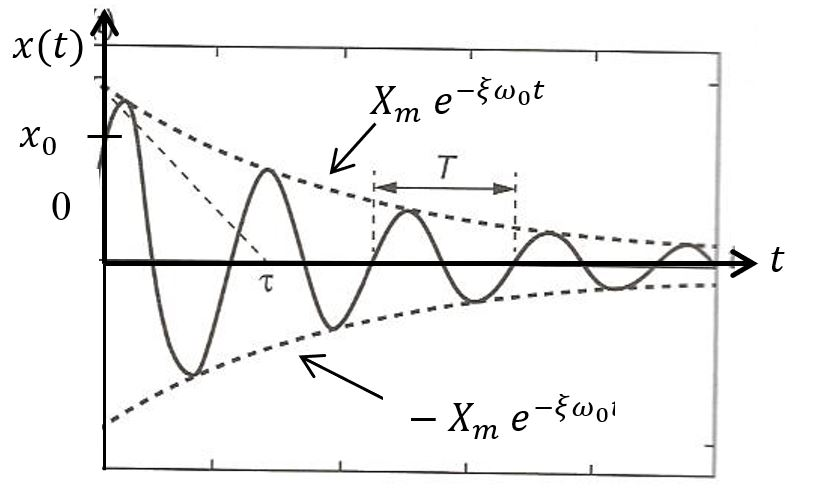
\includegraphics[width=.6\linewidth]{P2_corr}
\end{center}
}

\QR[1]{%
	Justifier qualitativement que l'énergie mécanique $\Ec(t)$ est une fonction
	décroissante de $t$. À quoi cela est-il dû~?
}{%
	À cause des frottements, l'énergie mécanique $\Ec(t)$ est une fonction
	décroissante de $t$.
}%

\QR[6]{%
	On envisage deux temps successifs $t_1$ et $t_2$ pour lesquels les
	déplacements sont $x_1$ et $x_2$, tels que $t_2 > t_1$ et $t_2-t_1=T$, où $T$
	est la période des oscillations amorties. En utilisant
	l'équation~\eqref{eq:cosfi} et en considérant que $\xi \ll 1$, montrer que~:
	\[
		\ln(\frac{x_1}{x_2}) \approx 2\pi\xi
	\]
}{%
	Cela fait penser au décrément logarithmique~:
	\begin{gather*}
		\delta =
		\ln\frac{x\left(t\right)}{x\left(t+T\right)} =
		\ln(\frac{x_1}{x_2}) \stm{=}
		\ln(\frac{%
				X_m\exr^{-\xi\w_0 t}\cos(\W t+\f)
			}{%
				X_m\exr^{-\xi\w_0 (t+T)}\cos(\W(T+t)+\f)
			})
		\stm{=} \ln(\exr^{\xi\w_0 T})
		\intertext{car cosinus est une fonction périodique de période $T$. Soit~:}
		\delta =
		\ln(\frac{x_1}{x_2}) \stm{=}
		\xi\w_0 T =
		\xi\w_0\frac{2\pi}{\W} =
		\xi\w_0\frac{2\pi}{\w_0\sqrt{1-\xi^2}}
		\Lra
		\boxed{\delta \stm{=} \xi\frac{2\pi}{\sqrt{1-\xi^2}}}
	\end{gather*}
	Or par hypothèse, $\xi \ll 1$, donc $1-\xi^2\approx 1$ \pt{1}~; alors
	\[
		\boxed{\ln(\frac{x_1}{x_2}) \stm{\approx} 2 \pi\xi}
	\]
}

\QR[10]{%
\noindent
\begin{minipage}[t]{.48\linewidth}
	Toujours dans le cas où $\xi\ll 1$, le relevé du déplacement horizontal de la
	plateforme en fonction du temps est représenté en figure 2 ci-dessous. En
	utilisant les deux points qui sont indiqués sur la figure 2, déterminer les
	valeurs numériques de $k$, $\xi$ et $\gamma$ (avec leurs unités). Comment ce
	tracé serait-il modifié si $\xi$ augmentait (un rapide graphique peut permettre
	d'être plus explicite)~?
\end{minipage}
\hfill
\begin{minipage}[t]{.48\linewidth}
	\vspace{0pt}
	\begin{center}
		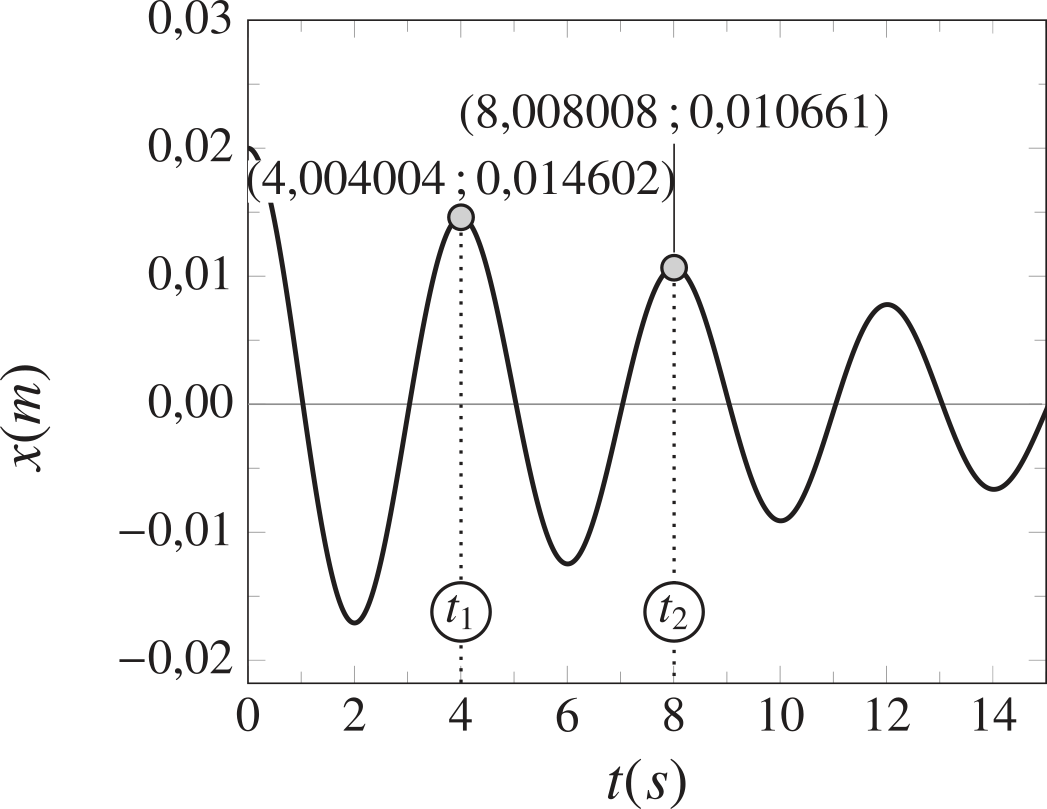
\includegraphics[width=\linewidth]{P2_graph}
		\captionof{figure}{Déplacement horizontal de la plateforme dans le temps.}
	\end{center}
\end{minipage}
}{%
On lit $x_1=\SI{0,014602}{m}$ et $t_1=\SI{4,004004}{s}$, puis
$x_2=\SI{0,010661}{m}$ et $t_2=\SI{8,008008}{s}$.
D'après l'énoncé, on a $T=t_2-t_1$ et comme $\xi \ll 1$ alors
\begin{gather*}
	\w_0 \stm{\approx} \W \stm{=} \frac{2\pi}{T} = \frac{2\pi}{t_2-t_1}
	\intertext{car $\W =\w_0\sqrt{1-\xi^2}$. De plus, $\w_0=\sqrt{\frac{k}{m}}$
		donc}
	\boxed{%
		k =
		m\w_0^2 \stm{=}
		m\frac{4\pi^2}{\left(t_2-t_1\right)^2}
	}%
	\Ra
	\xul{k \stm{=} \SI{2.71e5}{N.m^{-1}}}
	\\\beforetext{et}
	\boxed{\xi \stm{=} \frac{\ln (\frac{x_1}{x_2})}{2\pi}}
	\Ra
	\xul{\xi \stm{=} \num{5.01e-2}}
	\intertext{%
		On trouve en effet comme attendu $\xi\ll1$~: c'est cohérent.
	}%
	\beforetext{Enfin, d'après Q1,}
	\xi = \frac{\gamma}{2}\sqrt{\frac{1}{mk}}
	\\\beforetext{soit}
	\boxed{\gamma \stm{=} 2\xi\sqrt{mk}}
	\Ra
	\xul{\gamma \stm{=} \SI{1.73e4}{kg.s^{-1}}}
\end{gather*}
Si $\xi$ augmentait, l'amortissement augmenterait, la décroissance exponentielle
serait plus rapide, on verrait moins d'oscillations \pt{1}~; la pseudo-pulsation
$\W$ diminuerait et la pseudo-période $T={2\pi}/{\W}$ augmenterait. \pt{1}
}%

\end{document}
